\documentclass[border=3pt]{standalone}
% Preâmbulo compartilhado pelos diagramas TikZ da aula 5 de IHC (Processos de Design)
\usepackage[T1]{fontenc}
\usepackage[utf8]{inputenc}
\usepackage{lmodern}
\usepackage{amsmath}
\usepackage{xcolor}
\usepackage{tikz}
\usetikzlibrary{arrows.meta,angles,quotes,decorations.pathmorphing,calc,
                positioning,shapes.geometric,shapes.misc,backgrounds,fit,
                math}

% Paleta (mesma dos SVGs originais)
% Paleta da disciplina de IHC: acento roxo (#755099), da capa do livro.
% (o nome "dblue" é mantido para não alterar todos os diagramas)
\definecolor{dblue}{HTML}{755099}
\definecolor{dorange}{HTML}{B3541E}
\definecolor{dgreen}{HTML}{4A7C59}
\definecolor{dred}{HTML}{9C4B4B}
\definecolor{dcream}{HTML}{F4F1EA}
\definecolor{dshade}{HTML}{DDD7C9}

% Função gaussiana (não normalizada por padrão de escala visual)
\pgfmathdeclarefunction{gauss}{3}{%
  \pgfmathparse{1/(#3*sqrt(2*pi))*exp(-((#1-#2)^2)/(2*#3^2))}%
}

% Estilos comuns (prefixo d... para não colidir com chaves internas do pgf)
\tikzset{
  >={Stealth[length=2mm]},
  dguide/.style={gray!55, dashed, line width=0.4pt},
  daxis/.style={gray!60, line width=0.7pt, ->},
  dbody/.style={fill=black!3, draw=black!80, line width=1pt},
  dacc/.style={draw=dblue, line width=1pt},
  dlbl/.style={black!55, font=\small},
  dsub/.style={black!45, font=\footnotesize},
  dstate/.style={circle, draw=black!80, fill=dcream, line width=1pt,
                 minimum size=17mm, font=\large, inner sep=1pt},
  dobs/.style={circle, draw=black!80, fill=dshade, line width=1pt,
               minimum size=14mm, font=\large, inner sep=1pt},
  dbox/.style={rounded corners=2pt, draw=black!80, fill=dcream, line width=1pt,
               align=center, inner sep=6pt},
  dop/.style={circle, draw=black!80, fill=white, line width=1pt,
              minimum size=6mm, inner sep=0pt, font=\small},
  dtrans/.style={->, dblue, line width=1pt},
  dmeas/.style={->, dorange, line width=1pt},
  dcurve/.style={line width=1pt, dblue},
  dcurveb/.style={line width=1.4pt, dorange},
}

\begin{document}
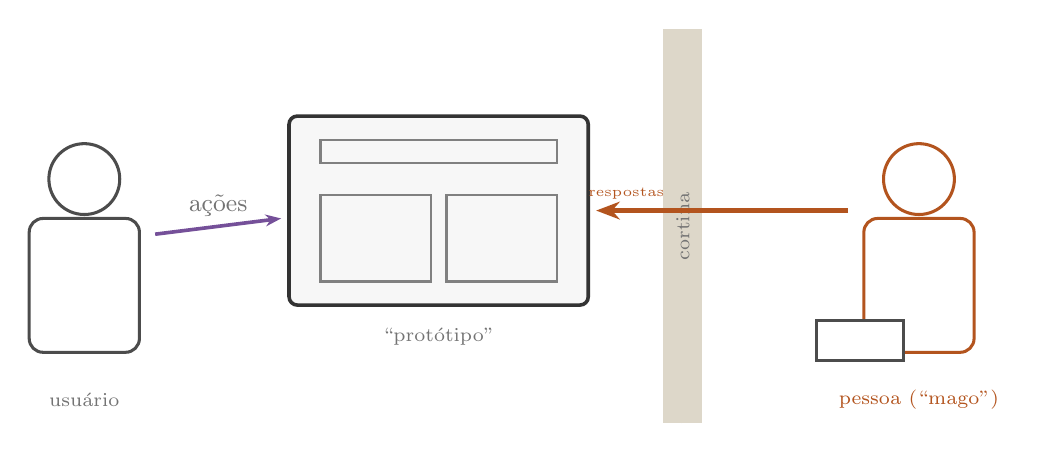
\begin{tikzpicture}[x=1cm,y=1cm]

  % usuário
  \draw[black!70, line width=1.1pt, fill=white] (0,2.5) circle (0.45);
  \draw[black!70, line width=1.1pt, fill=white, rounded corners=5pt] (-0.7,0.3) rectangle (0.7,2.0);
  \node[dlbl, font=\scriptsize] at (0,-0.3) {usuário};

  % tela
  \draw[dbody, line width=1.3pt, rounded corners=3pt] (2.6,0.9) rectangle (6.4,3.3);
  \draw[black!50, line width=0.8pt] (3.0,2.7) rectangle (6.0,3.0); \draw[black!50, line width=0.8pt] (3.0,1.2) rectangle (4.4,2.3); \draw[black!50, line width=0.8pt] (4.6,1.2) rectangle (6.0,2.3);
  \node[dlbl, font=\scriptsize] at (4.5,0.5) {``protótipo''};
  \draw[dtrans, line width=1.3pt] (0.9,1.8) -- (2.5,2.0) node[midway, above, font=\tiny, dlbl] {ações};

  % cortina
  \draw[black!40, dashed, line width=1.3pt] (7.6,-0.6) -- (7.6,4.4);
  \fill[dshade] (7.35,-0.6) rectangle (7.85,4.4);
  \node[dlbl, font=\scriptsize, rotate=90] at (7.6,1.9) {cortina};

  % mágico
  \begin{scope}[shift={(10.6,0)}]
    \draw[dorange, line width=1.1pt, fill=white] (0,2.5) circle (0.45);
    \draw[dorange, line width=1.1pt, fill=white, rounded corners=5pt] (-0.7,0.3) rectangle (0.7,2.0);
    \node[dlbl, font=\scriptsize, dorange] at (0,-0.3) {pessoa (``mago'')};
    \draw[black!70, line width=1pt, fill=white] (-1.3,0.2) rectangle (-0.2,0.7);
  \end{scope}
  \draw[dmeas, line width=1.5pt, -{Stealth[length=3mm]}] (9.7,2.1) -- (6.5,2.1) node[pos=0.88, above, font=\tiny, dorange] {respostas};


\end{tikzpicture}
\end{document}
